\documentclass[11pt,letterpaper]{article}
\usepackage{tikz}
\usepackage{wrapfig}
\usepackage{amsmath}
\usepackage{comment}
\usepackage{xcolor}
\usepackage[backend=biber, style=ieee]{biblatex} 
\addbibresource{midterm_report/assets/refs.bib}
\usepackage[utf8]{inputenc}
\usepackage{graphicx}
\usepackage{float}  
\usepackage{fullpage}
\usepackage{algorithm}
\usepackage{algpseudocode}
\usepackage{subcaption}
\usepackage{listings}
\usepackage{xcolor}
\usepackage{wrapfig}
\usepackage{float}            % for [H]
\usepackage[section]{placeins} % for \FloatBarrier


% Define code style
\lstdefinestyle{pythonstyle}{
    backgroundcolor=\color{gray!10},   % Background color
    commentstyle=\color{green},        % Comment style
    keywordstyle=\color{blue},         % Keyword style
    numberstyle=\tiny\color{gray},     % Line numbers style
    stringstyle=\color{orange},        % String style
    basicstyle=\ttfamily\footnotesize, % Basic font style
    breaklines=true,                   % Line breaking
    frame=single,                      % Frame around the code
    numbers=left,                      % Line numbers on the left
    captionpos=b,                      % Caption at the bottom
    showstringspaces=false             % Hide spaces in strings
}

\lstset{style=pythonstyle}

\begin{document}


\title{DeClip: Hard Negative Mining through Image Decomposition and Inpainting}


\author{
Zhanhao Liu (zhanhaol@umich.edu),
Huanchen Jia (jhuanch@umich.edu),\\
Qiulin Fan (rynnefan@umich.edu),
Lingyu Meng (jmly@umich.edu)\\
}

\date{05/01/2025}


\maketitle
\begin{center}
    \section*{Abstract}
\end{center}
Contrastive Language–Image Pretraining(CLIP) excels in multimodal learning, enabling zero-shot classification, cross-modal retrieval, and transfer learning. However, its reliance on global image-text alignment limits its ability to capture localized features, weakening performance in fine-grained visual tasks.\cite{liu2024an} To address this, DeClip introduces image-based hard negatives by modifying key image-caption pairs, enhancing model robustness and discrimination. This improves CLIP’s ability to distinguish fine-grained details, strengthening its effectiveness in contrastive learning and multimodal tasks.\\
\section{Introduction}
\begin{figure}[h]
    \centering
    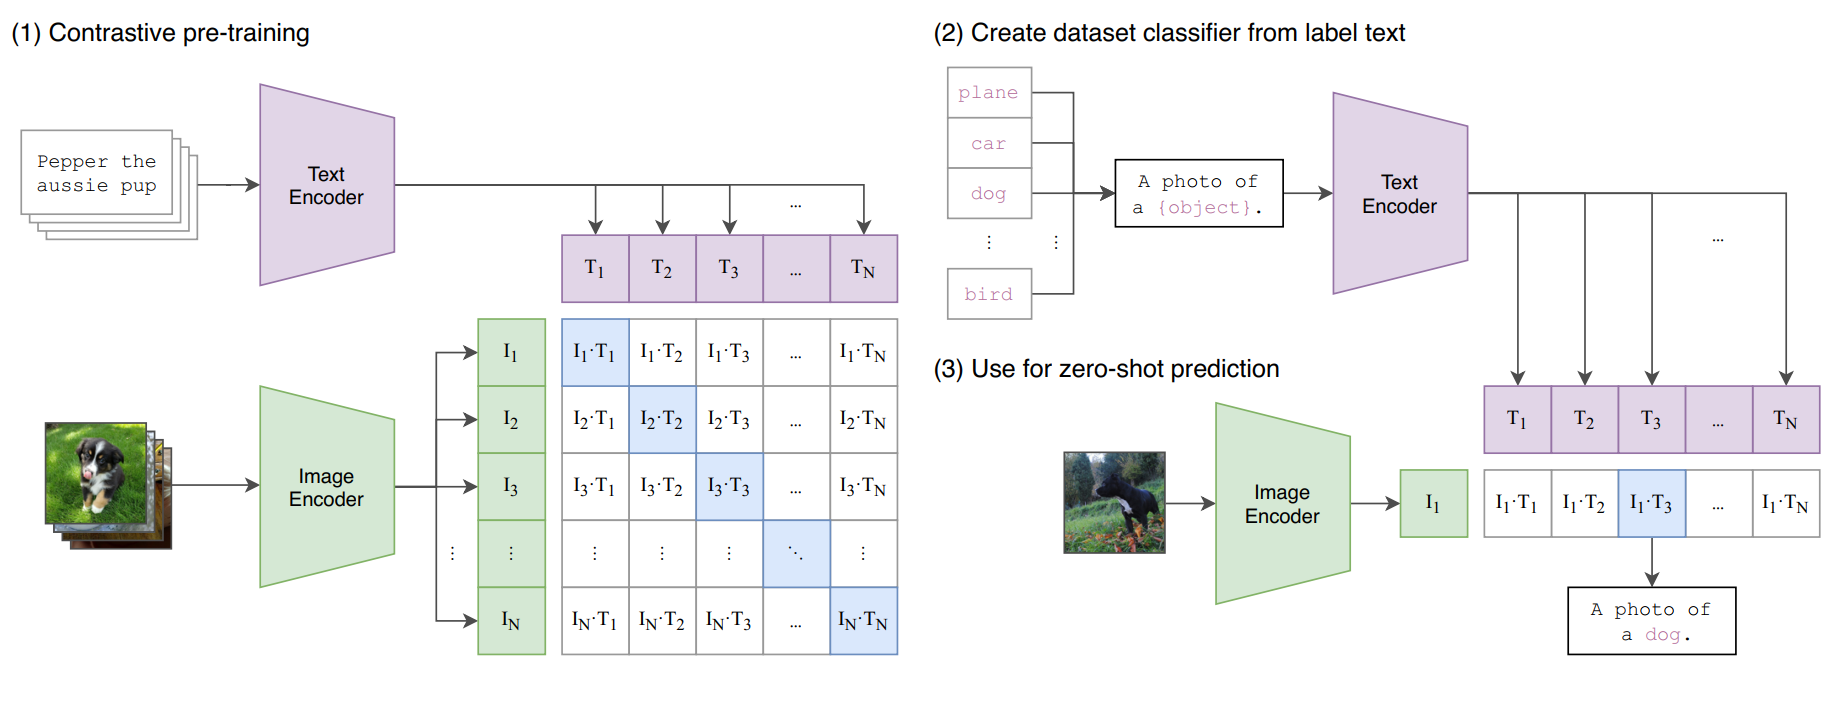
\includegraphics[width=0.65\linewidth]{final_report/assets/openai_clip.png} 
    \caption{Original CLIP Model}
    \label{fig:Original_CLIP_Model}
\end{figure}

CLIP\cite{radford2021learningtransferablevisualmodels} (Radford et al., 2021), trained on full images, struggles to learn localized features due to its reliance on global image-text alignment, limiting its effectiveness in fine-grained visual-text tasks like object classification and caption-based retrieval. This limitation hinders its ability to capture subtle visual differences, which is especially problematic in safety-critical domains such as medical imaging and robotics, where precise distinctions—like identifying diseased tissue or ensuring accurate tool positioning—are crucial. Solving this problem would improve CLIP’s ability to learn localized visual details, enhancing its adaptability to tasks requiring fine-grained reasoning and ultimately making it more effective in real-world multimodal applications.

\vfill
\noindent\tiny\url{https://github.com/SaddySamoyed/545-project}
\normalsize

\FloatBarrier 

\section{Proposed method}
\subsection{Overall Approach}
We propose DeCLIP, an image-side hard negative mining architecture as a way to enhance CLIP’s attention to fine-grained features and improve its robustness in real-world multimodal tasks. 

Prior research suggests that, for each pair of correct (image, caption) example, by rewriting the caption, e.g. reordering and changing its constituents, we can generate into a hard negative. (Fan, Krishnan, et. al.\cite{fan2023improvingcliptraininglanguage}). Our idea has similarities and extensions. 

For each ground-truth pair \((I, C)\), we remove certain key visual components (e.g.\ the main object or salient regions) from the image \(I\), yielding \(I'\) that remains highly similar in low-level appearance yet no longer matches its original caption \(C\), thus forming a hard negative for contrastive learning. Simultaneously, we excise the corresponding keywords from the caption \(C\) to create a modified caption \(C'\) as a new positive example, reinforcing the model’s sensitivity to missing information. We prioritize the image side because the visual embedding manifold is both higher-dimensional and exhibits superior topological smoothness, allowing fine-grained decomposition and recomposition of localized features that text-only perturbations cannot capture. Although constructing image-level hard negatives incurs greater computational and annotation cost compared to text-level augmentations, it significantly amplifies sample diversity and robustness—especially on small datasets—yielding more discriminative vision–language alignment than text-only methods.


\begin{figure}{}
    \centering
    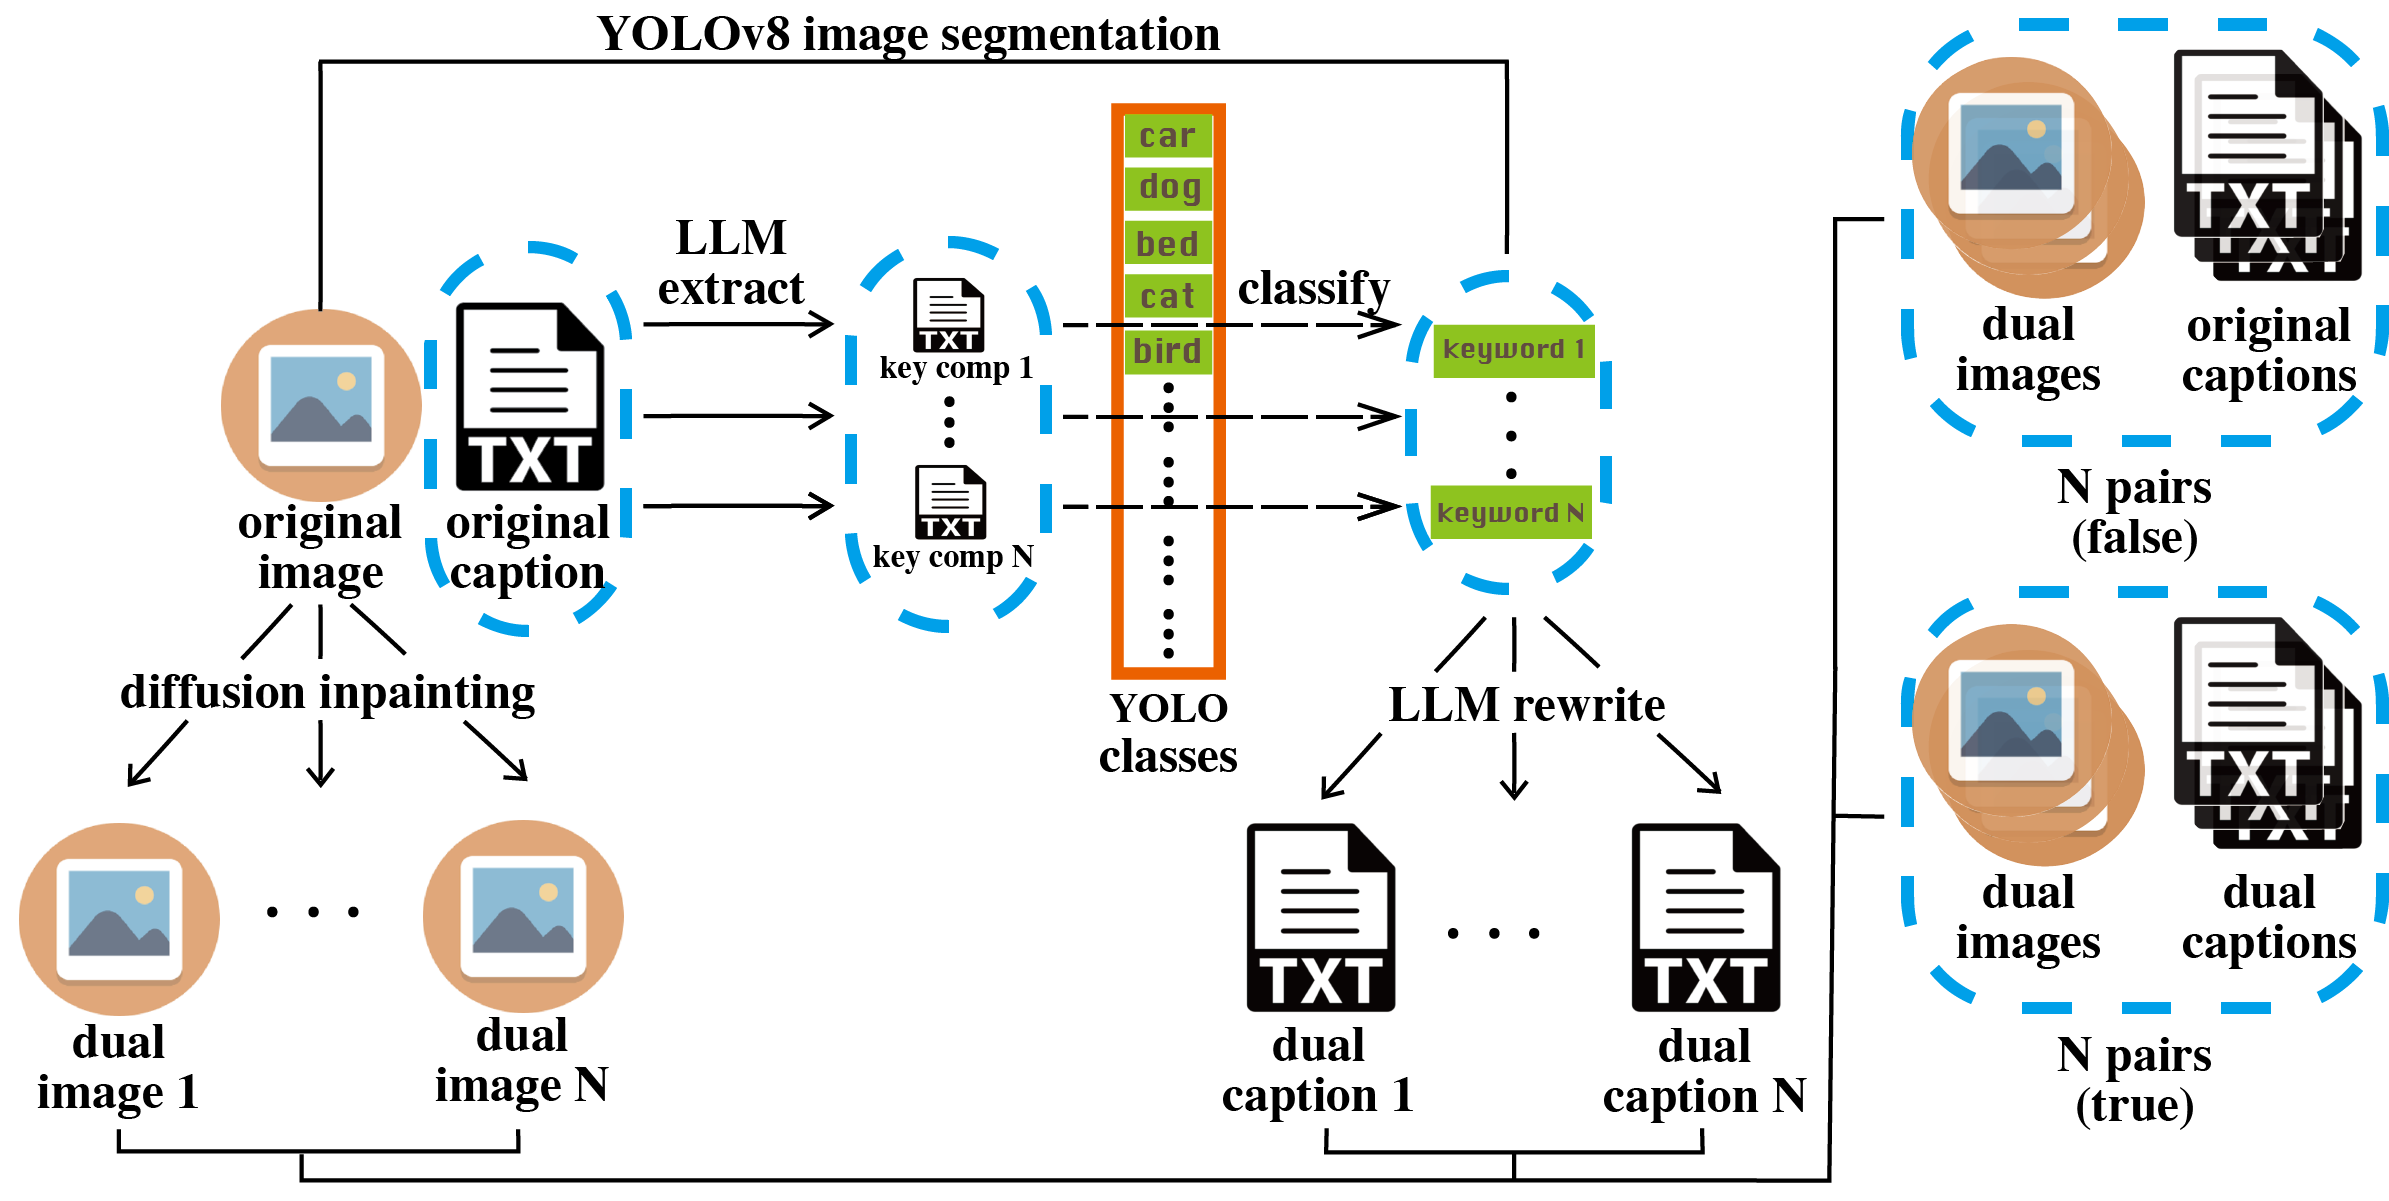
\includegraphics[width=0.9\textwidth]{final_report/assets/overall_method.png}
    \caption{Overall approach}
\end{figure}


Given an image-text pair:
\begin{itemize}
    \item Removing a key object from the image creates a new image we call \textbf{dual image}, together with the caption unchanged → a semantically mismatched hard negative.
    \item Removing corresponding keywords from the caption creates a new caption we call \textbf{dual caption}, together with the altered image → a new positive pair.
\end{itemize}

% Surely, dual images and original captions form false examples and almost surely, dual images and dual captions form negative examples. 

Below is our algorithm in concrete:
\begin{algorithm}[H]
\caption{Generating Dual Image-Caption Pairs via Component Removal}
\begin{algorithmic}[1]
\State \textbf{Input:} Batch size $K$, data $\{(I_i, C_i)\}_{i=1}^K$, pretrained LLM, segmentation model (e.g., YOLOv8), diffusion inpainting model
\State \textbf{Hyperparameter:} Number of key components to extract $N$ (e.g., $N = 3$)
\For{$i = 1$ to $K$}
        \State \textbf{Step 1:} Use LLM to extract up to $N$ key components from caption $C_i$
        \State Classify extracted keywords into predefined object classes, forming a keyword-class map
    \For{$n = 1$ to $N$}
        \State \textbf{Step 2:} Try to detect the $n^{\text{th}}$ component in image $I_i$ using a segmentation model
        \If{detection succeeds}
            \State Save mask $M_{i,n}$ for component $n$
        \Else
            \State Remove the $n^{\text{th}}$ keyword-class mapping from the keyword map, continue
        \EndIf
    \EndFor
    \For{$n = 1$ to $N$}
        \State \textbf{Step 3:} Use diffusion model to remove component $n$ by applying mask $M_{i,n}$ to $I_i$, producing $I_{i,n}'$
    \EndFor
    \For{$n = 1$ to $N$}
        \State \textbf{Step 4:} Use LLM to remove keyword $n$ from caption $C_i$, producing dual caption $C_{i,n}'$
    \EndFor
\EndFor
\State \textbf{Output:} $\{(I_{i,n}', C_{i,n}')\}_{i=1,\ldots,K}^{n=1,\ldots,N}$ — Dual image-caption pairs with one component removed
\end{algorithmic}
\end{algorithm}

\subsection{Reasonability of the Idea}

\begin{wrapfigure}{r}{0.45\textwidth}  % 'r' 表示右侧,宽度可调
  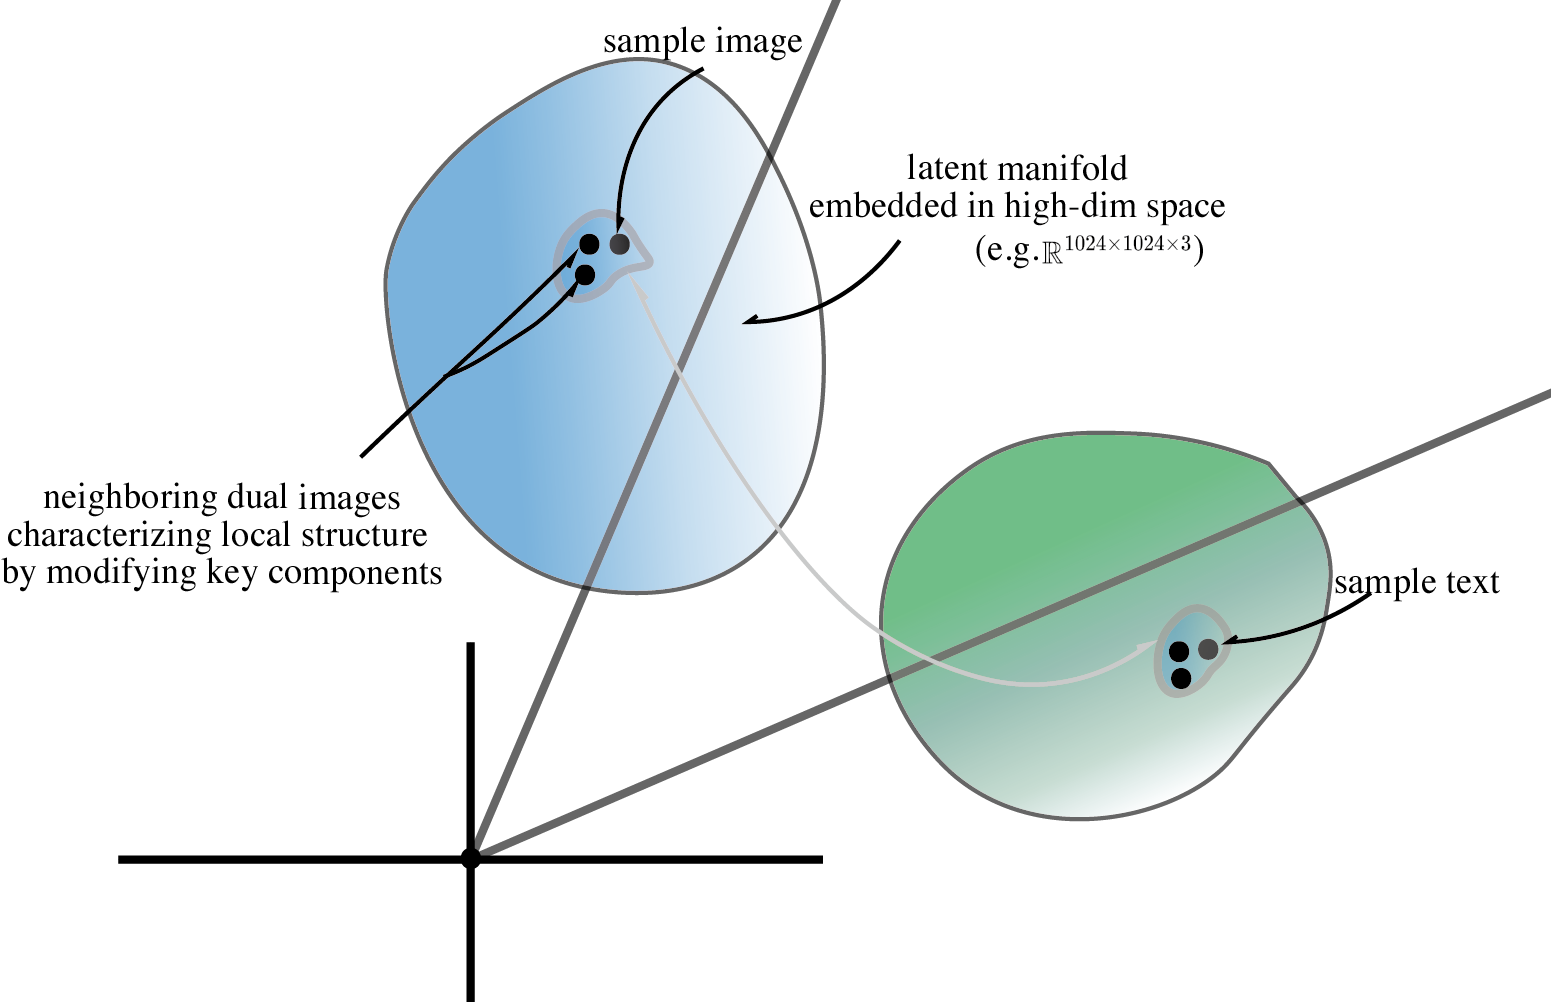
\includegraphics[width=0.5\textwidth]{final_report/assets/manifold.png}  % 替换为你的图片路径
  \caption{embedding data manifold of CLIP space}
\end{wrapfigure}
Our idea invokes the manifold hypothesis, aims at improving CLIP's composition-reasoning ability. Prior work has shown that the embedding manifold of CLIP is characterized as double-ellipsoids\cite{levi2024doubleellipsoidgeometryclip} (Levi, Gilboa, 2024), and we hypothesize: dual images with critical components removed characterize the local structure of the original image, as a valid interpolation; and the generation of dual texts can let the model learn the mapping between the sample image and the open neighborhood near the caption. We conjecture that our approach increases the combinatorial inference ability and robustness of the model on training with small datasets.




\begin{comment}
  \begin{center}
    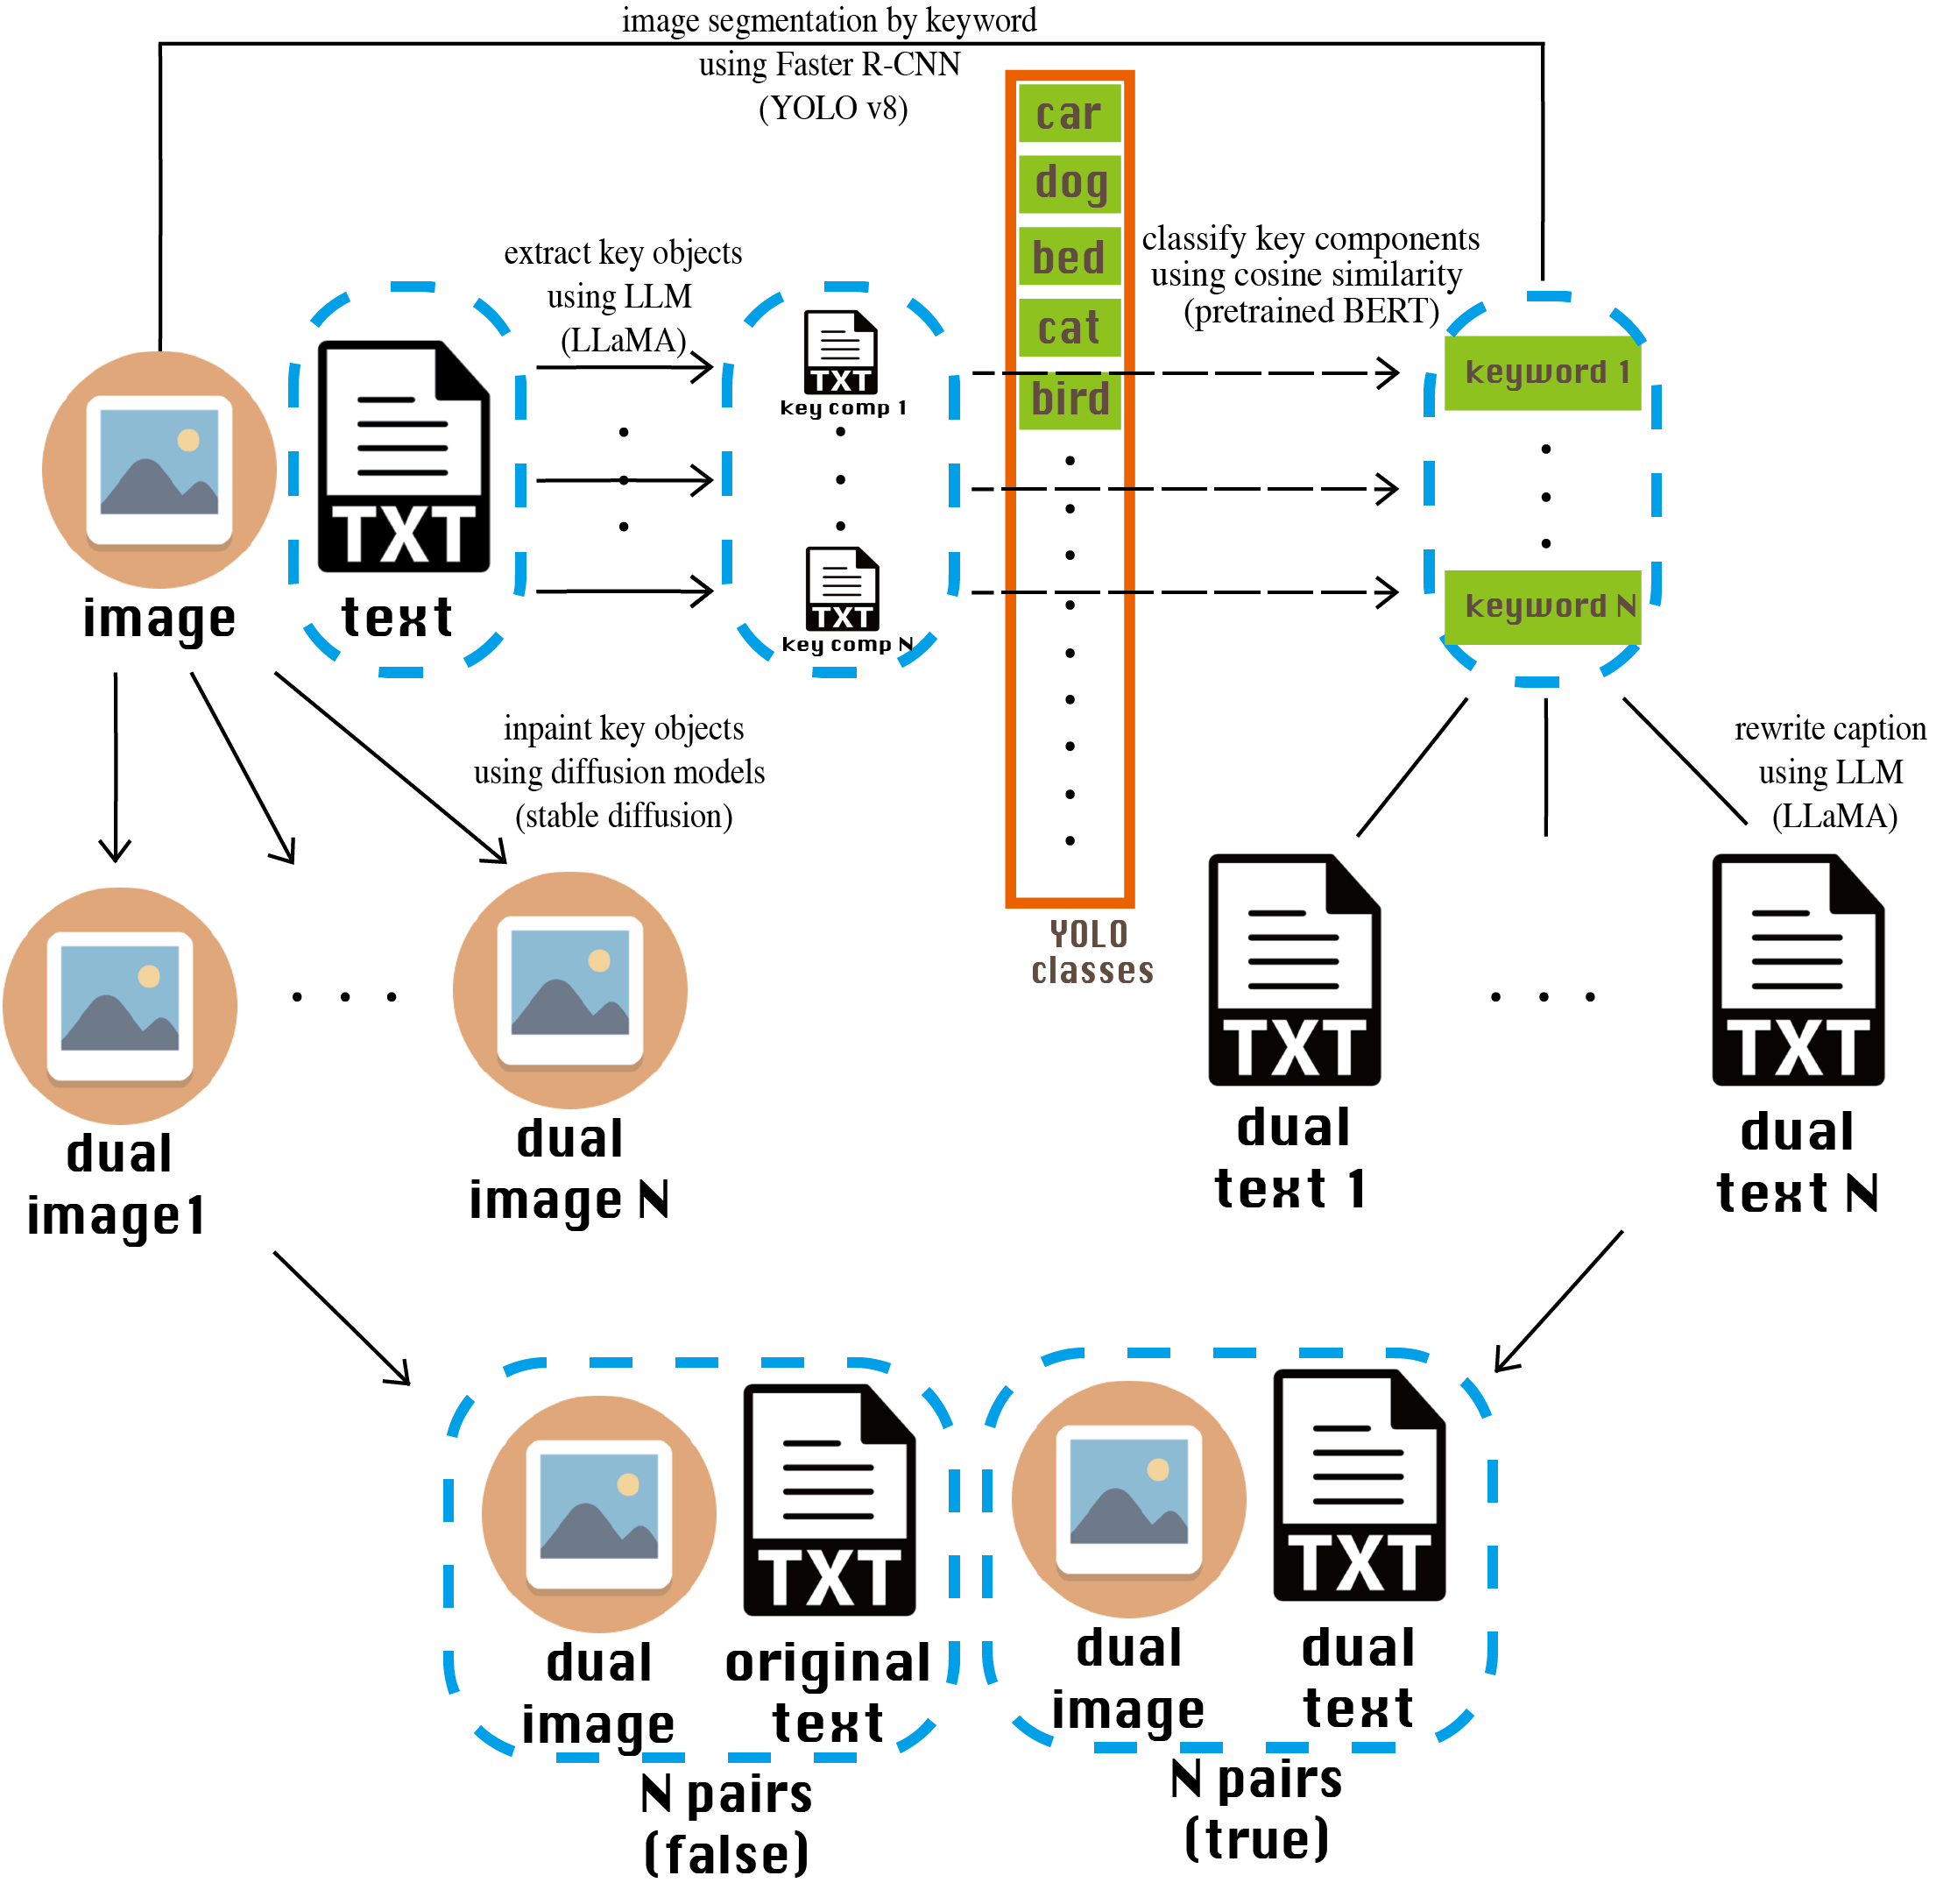
\includegraphics[width=1\textwidth]{midterm_report/pipeline.png} 
\end{center}
\end{comment}




\section{Related work}
\subsection{Existing Methods:}
 CLIP's performance is shown recently that it could be enhanced by leverging the difficulty in training.\\
Currently the exisiting methods mostly improve in the following perspectives.\\
\begin{itemize}
    % \item \textbf{Hard Negative Mining}: Hard negative examples are those that are semantically similar to the positive samples but belong to different classes, making it challenging for the model to distinguish between them. In contrastive learning, two primary strategies enhance model performance: generation-based methods and regularization-based methods. Generation-based methods, such as NegCLIP and SVLC, create hard negatives by altering positive samples to produce semantically similar yet incorrect pairs, challenging models to discern subtle differences. Regularization-based methods employ strategies like intra-modal contrastive loss and ranking cross-modal hard negatives to refine learning.

    \item \textbf{Hard Negative Mining}: Hard negatives closely resemble positive samples yet belong to different classes, making them difficult to distinguish. In contrastive learning, two main strategies address this: generation-based and regularization-based. Generation-based methods (e.g., NegCLIP\cite{yuksekgonul2023visionlanguagemodelsbehavelike} ((Yuksekgonul et al., 2022)) modify positive samples to create semantically similar but incorrect pairs, forcing models to learn subtle distinctions. Regularization-based methods use techniques like intra-modal contrastive loss and cross-modal ranking of hard negatives to refine learning.

    
    
    \item \textbf{Fine-Grained Cross-Modal Alignment Fine-Tuning}: Some previous works such as FILIP\cite{yao2021filipfinegrainedinteractivelanguageimage} (Yao et al., 2021) enhances multimodal alignment by matching local image patches with specific text tokens via a similarity matrix. Unlike CLIP’s global image-text matching, it computes token-level contrastive losses, forcing visual and textual tokens to mutually select their most relevant counterparts. The regional information and details could be better learned this way.
\end{itemize}
DeCLIP combines the idea of \textbf{Hard Negative Mining} and \textbf{Fine-Grained Cross-Modal Alignment Fine-Tuning} such that the model can deepen its understanding of the entire image by paying attention to the regional changes of the image. DeCLIP is different from existed \textbf{Hard Negative Mining} in applying the changes to \textbf{images} instead of \textbf{texts}, while it is improved based on \textbf{Fine-Grained Cross-Modal Alignment Fine-Tuning} by considering contexts of texts and layout of images
\subsection{Core Model and Tool References:}
Our framework integrates state-of-the-art multimodal tools. For text extraction, we query GPT-4o to identify key noun words from the caption. We then map these nouns to $80$ specified catogories of \texttt{yolov8n-seg.pt}. This whole process is also conducted by GPT-4o. For image segmentation, \texttt{yolov8n-seg.pt} \cite{ultralytics2023segment} (Ultralytics, 2025)(a lightweight YOLOv8 variant pretrained on COCO) is used.\\ Inpainting leverages \texttt{runwayml/stable-diffusion-inpainting} \cite{stabilityai2023inpainting}(Stable-diffusion-v1-5/Stable-diffusion-inpainting · Hugging Face, n.d.) and \texttt{CLIP}, ensuring robust image–text understanding.



\section{Pipeline Instance Demonstration}
We have designed and implemented a pipeline that generates hard negative samples by removing key visual objects from an image and rewriting the associated caption accordingly. The resulting (image, caption) pairs enhance the CLIP model’s ability to distinguish subtle, localized visual-text misalignments. This section presents an example of our four-step procedure.
\begin{figure}[h]
    \centering
    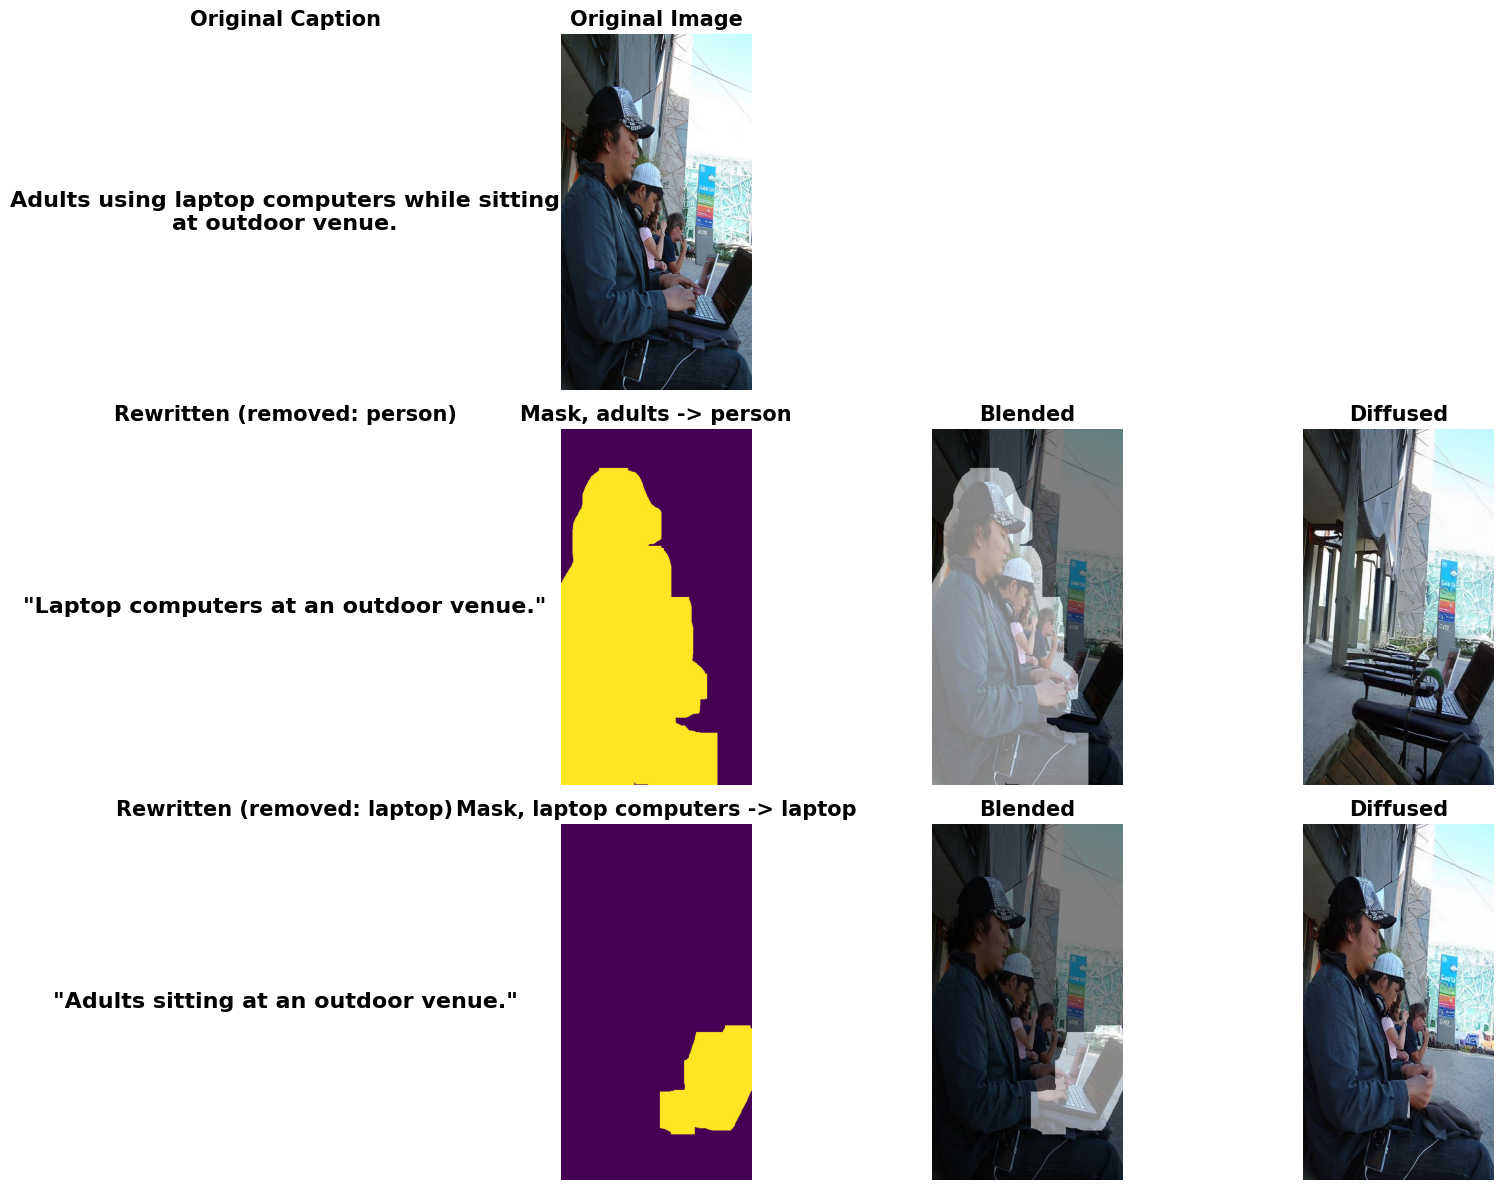
\includegraphics[width=0.85\textwidth]{final_report/assets/preliminary.png}
    \caption{{A random sample of dual (image, caption) pairs generated by DeCLIP. The left column shows the original image and caption. The middle columns show object-level masks (e.g., person, laptop) and corresponding rewritten captions. The right columns show inpainted images after object removal.}}
    \label{fig:preliminary_pipeline}
\end{figure}

\paragraph*{Step 1: Caption Parsing and Key Term Extraction}
\textbf{Method:} We use GPT-4o to extract noun phrases from the caption. Multi-word expressions like ``laptop computers'' are treated as single semantic units.
\noindent
\textbf{Example:}
\begin{itemize}
  \item \textcolor{black}{Extracted Terms: ``adults'', ``laptop computers'', ``outdoor venue''}
\end{itemize}

\paragraph*{Step 2: Mapping Phrases to Object Categories}
\textbf{Method:} Extracted phrases are matched to YOLOv8\cite{ultralytics2023segment} object categories using LLM-rewrite. Phrases that cannot be reliably mapped or detected are discarded.
\noindent
\textbf{Example:}
\begin{itemize}
  \item \texttt{adults} $\to$ \texttt{person}, \texttt{laptop computers} $\to$ \texttt{laptop}
\end{itemize}

\paragraph*{Step 3: Object Detection and Mask Generation}

\textbf{Method:} YOLOv8 segmentation detects the target objects and produces binary masks. Each mask isolates a specific object (e.g., person or laptop) for subsequent inpainting.

\paragraph*{Step 4: Object Removal and Caption Rewriting}

\textbf{Method:} Detected objects are removed from the image using a Stable Diffusion inpainting model\cite{stabilityai2023inpainting}. Simultaneously, the caption is modified by removing the corresponding phrase, forming the ``dual caption''.

\noindent
\textbf{Resulting Pairs:}
\begin{itemize}
    \item {Original: ``Adults using laptop computers while sitting at outdoor venue.''}
    \item {Dual 1: ``Laptop computers at an outdoor venue.'' (person removed)}
    \item {Dual 2: ``Adults sitting at an outdoor venue.'' (laptop removed)}
\end{itemize}


\noindent
\section{Fine-tune}

We explored several strategies for adapting CLIP to our specialized, localization‐focused dataset. First, we attempted full‐parameter fine-tuning but found that, given our relatively small training set, this led to overfitting and degraded generalization. To address this, we froze all of CLIP’s weights except the top three transformer layers of the text encoder and the top six layers of the visual encoder. This partial‐freeze scheme preserves CLIP’s broad, pretrained representations while providing capacity for learning finer, localized patterns.
Because our “dual” images share high‐level semantics with the originals but differ only in localized details, we found it counterproductive to push their embeddings arbitrarily far apart. Instead, we introduce a dual‐caption hinge loss that penalizes precisely two error modes:

\begin{itemize}
  \item[1.] when a dual image is more similar to the original caption than the true image is, and
  \item[2.] when a dual caption is more similar to the original image than the true caption is.
\end{itemize}


This targeted penalty encourages CLIP to focus on the subtle, localized differences encoded by our dual examples without overriding its general alignment. Finally, we combine this hinge term with the standard CLIP cross‐entropy loss (InfoNCE) so that the model retains its pretrained zero-shot retrieval performance even as it acquires new, location‐sensitive discriminative ability.
  Notation setup for sample \(i\):
    \begin{itemize}
      \item[\(\,1.\)] \(v_i\): normalized embedding of the true image.
      \item[\(\,2.\)] \(t_i\): normalized embedding of the true caption.
      \item[\(\,3.\)] \(D_i = \{d_{i,1}, \ldots, d_{i,M_i}\}\): normalized embeddings of the dual captions.
      \item[\(\,4.\)] \(N_i = \{n_{i,1}, \ldots, n_{i,M_i}\}\): normalized embeddings of the negative images.
    \end{itemize}

\begin{equation}
\mathcal{L}_{\text{dual},i} = \sum_{k=1}^{M_i} \max\left(0, sim(v_i, d_{i,k}) - sim(v_i, t_i)\right).
\end{equation}

\begin{equation}
\mathcal{L}_{\text{neg},i} = \sum_{j=1}^{M_i} \max\left(0, sim(n_{i,j}, d_{i,j}) - sim(n_{i,j}, t_i)\right).
\end{equation}

\FloatBarrier 








\section{Result}
\begin{table}[ht]
\centering
\caption{Zero-shot Performance to cifar10 and ARO}
\begin{tabular}{|l|c|c|}
\hline
\textbf{Method} & \textbf{Zero-shot on cifar10} & \textbf{ARO} \\ \hline
base clip       & 0.1845              & -            \\ \hline
Tuned clip & 0.1876              & 0.49129553       \\ \hline
D-dip           & 0.1964              & 0.49881730       \\ \hline
\end{tabular}
\end{table}

To set up our experiments, we first trained CLIP from scratch for a limited number of epochs to establish a base model. We then fine-tuned this base model on the original dataset - this variant is referred to as \textbf{Tuned CLIP}. In parallel, we fine-tuned the same base model on our generated dual-image/dual-caption dataset, yielding the \textbf{D-CLIP} model for comparison. Notably, because we filtered out unhelpful objects from the captions, roughly 30 \% of the images in the original dataset could not be paired with a corresponding dual image and caption. As a result, the dataset used to train D-CLIP is significantly smaller than the one used to train Tuned CLIP.

The results show better performance for D-CLIP compared with the Tuned clip in Cifar 10, indicating that our dataset has helped CLIP enhance its general ability while learning localized features. In the ARO benchmark, D-CLIP shows a slight increase in accuracy over the Tuned clip. Although the improvement is modest, D-CLIP is trained on a smaller dataset than the Tuned clip - only 70\% of the original examples were used for dual generation. This demonstrates that, with our dataset, we can achieve similar or better results with reduced storage and computational costs. Given the size of our training data, we believe the results provide a convincing signal that our pipeline successfully enhances the CLIP model’s localized feature learning and general performance.




% The base CLIP’s failure on ARO (–) highlights a gap between general representation quality (0.1845) and relational reasoning. S-epoch CLIP’s boost (0.6716→0.4983) suggests that extended epoch tuning enhances relational alignment. Notably, D-dip matches S-epoch’s ARO (0.4988) despite its low base metric (0.1964), indicating that targeted interventions like hard-negative mining can sharpen relational reasoning independently of overall performance gains. These results demonstrate that specialized interventions may more efficiently improve relational reasoning than simply scaling general training.

\section{Limitations}
\subsection{Time and Computational Cost Analysis}
Generating dual examples scales linearly with dataset size but remains dominated by diffusion sampling. On an A100 GPU we process 1 000 COCO images at a time and observe \approx59 min per batch (\approx 3.54 s per image–caption pair, of which \approx 2.9 s is diffusion). Projected to all 82 783 COCO training examples, dual data generation takes \approx 81.4 hours. For larger collections, lighter generators (e.g. VAE-based) will be needed to trade off image quality against run time.

\subsection{Limitation of Performance by Error Labelling}
Since our fine-tuning relies on automatically generated “dual” examples, a small fraction of labels can be incorrect. Two main error modes arise:
\begin{itemize}
    \item Diffusion hallucinations: the model sometimes inserts an unrelated object into the background, breaking the intended mismatch.
    \item Over‐reduction in captions: when the original caption contains only nouns, removing it leaves almost no content, so the LLM resorts to generic rewrites (e.g. “a man” → “somebody”) that fail to change semantics.
\end{itemize}

\subsection{Forgetting Previously Learned Information}
Since our model is intentionally trained to distinguish images and captions based on only subtle feature changes, there is a risk of disrupting CLIP’s original capabilities.


\section{Conclusion}
In this work, we developed a caption-guided object removal pipeline that leverages YOLOv8-based object detection, stable diffusion inpainting, and large language models to extract key objects from image-caption pairs, classify them into predefined categories, and generate precise masks for targeted object removal. By modifying images, while preserving structural relevance, we created hard negative images that misalign with their original captions, enhancing contrastive learning in CLIP-based models and improving their ability to distinguish fine-grained differences between text and images. Additionally, the altered images were incorporated into the training dataset as false samples to fine tune the existing model. Our model was tested on CIFAR-10 and the ARO benchmark, and it demonstrated convincing results. While our approach demonstrates the feasibility, future work should focus on refining object classification, supporting multi-object handling, and scaling data generation to improve DeClip’s effectiveness in multimodal learning.

\section{Future Plan}
\begin{itemize}
    \item We will need to automate the procedure for relatively large dataset (e.g. 3 million images), requiring the balance between efficiency and quality of inpainting, otherwise we might introduce noisy generated images. So we need to tweak the tech stack and architecture slightly after practice.
    \item We will further optimize the structure: if a class of examples are already well-learned, then we do not need to improve the accuracy of shotting concerning images. We will not generate $2N$ new examples for all existing examples, but reselect a subset of all images in a dataset for computation cost.
\end{itemize}

\section*{Contribution}
\begin{itemize}
    \item \textbf{Zhanhao Liu} 
    \begin{itemize}
        \item Implemented the \emph{word matching} and \emph{Stable Diffusion} code.
        \item Develop multiple fine-tuning methods and train CLIP model
        \item Conduct experiments and benchmarks 
    \end{itemize}
    \item \textbf{Huanchen Jia} 
    \begin{itemize}
        \item Researched state-of-the-art methods and reviewed the literatures for the group.
        \item Implemented the \emph{noun extraction} and \emph{compound word emerging} and \emph{LLM-rewrite} code.
        \item Data generation and organization for the model to process.
    \end{itemize}
    \item \textbf{Qiulin Fan} 
    \begin{itemize}
        \item Conceived the idea and drawed the demonstration images
        \item Implemented the \emph{object detection, mask generation and blend demonstration} code.
        \item         Stringed together the code in the pipeline, and written debugs
    \end{itemize}
    \item \textbf{Lingyu Meng} 
    \begin{itemize}
        \item Researched \emph{datasets and benchmarks} for future work.
        \item Organize the overall project content and design the poster layout

    \end{itemize}
\end{itemize}

\printbibliography


\appendix

\end{document}